\section{Validación}
Para la realización de la validación se implementó la clase Analisis, donde se crearon los objetos necesarios de los tipos Metal, Muestra, Reporte. Además, se implementó los métodos para su creación y adecuado funcionamiento.

\begin{lstlisting}
class Analisis

types
public String = seq of char;

instance variables
private metales: seq of Metal;
private muestras: seq of Muestra;
private reportes: seq of Reporte;
private limites: map int to Metal;
private peligro: seq of String;

operations
public Analisis: () ==> Analisis
Analisis() == ();

public valoresPrueba1: () ==> () 
valoresPrueba1() == (
	limites := {1 |-> new Metal(1, "Plomo", 10.0), 2 |-> new Metal(2, "Mercurio", 6.0), 3 |-> new Metal(3, "Arsénico", 4.0)};
	metales := [new Metal(1, "Plomo", 12.5), new Metal(2, "Mercurio", 5.0), new Metal(3, "Arsénico", 3.2)];
	muestras := [new Muestra(1, "Laboratorio A", mk_(2024, 10, 20), mk_(14, 30, 0), [metales(1), metales(2)]), new Muestra(2, "Laboratorio B", mk_(2024, 10, 21), mk_(16, 0, 0), [metales(2), metales(3)])];
	reportes := [new Reporte(1, limites, muestras, false), new Reporte(2, limites, muestras, false)];
);

public valoresPrueba2: () ==> () 
valoresPrueba2() == (
	limites := {1 |-> new Metal(1, "Plomo", 10.0), 2 |-> new Metal(2, "Mercurio", 6.0),  3 |-> new Metal(3, "Arsenico", 4.0)};
	metales := [new Metal(1, "Plomo", 4.5), new Metal(2, "Mercurio", 5.0), new Metal(3, "Arsenico", 3.2)];
	muestras := [new Muestra(1, "Laboratorio A", mk_(2024, 09, 20), mk_(14, 30, 0), [metales(1), metales(2)]), new Muestra(2, "Laboratorio B", mk_(2024, 10, 21), mk_(16, 0, 0), [metales(2), metales(3)])];
	reportes := [new Reporte(1, limites, muestras, false), new Reporte(2, limites, muestras, false)];
);

public ejecutarAnalisis: () ==> String
ejecutarAnalisis() == (
  for all reporte in set elems reportes do (
    if reporte.riesgoMetal() then
		return "PELIGRO! CONCENTRACION DANINA";
  );
  return "SITUACION SEGURA";
);

end Analisis
\end{lstlisting}


A continuación, se presenta el uso de la clase Analisis, para la ejecución de las pruebas establecidas de funcionamiento del Sistema de Detección.
\begin{figure}[h]
    \centering
    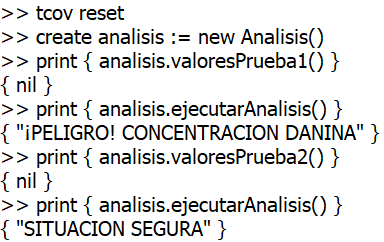
\includegraphics[width=0.5\textwidth]{Recursos/RealizandoPruebas.png}
    \caption{Realizando Pruebas con la clase Analisis.}
\end{figure}


Por consiguiente, se presenta la construcción del Coverage de las clases de nuestro Sistema de Detección, la cual consta de un 100\%. Para ello, se muestra la primera parte de los resultados del Coverage.
\begin{figure}[h]
    \centering
    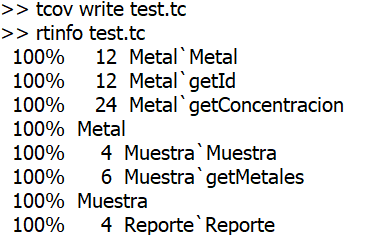
\includegraphics[width=0.5\textwidth]{Recursos/AnalisisCoverage1.png}
    \caption{Realizando Analisis de Coverage, Parte 1.}
\end{figure}

Finalmente, se muestra la segunda parte de los resultados del Coverage del Sistema de Detección.

\begin{figure}[h]
    \centering
    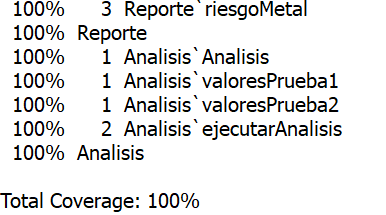
\includegraphics[width=0.5\textwidth]{Recursos/AnalisisCoverage2.png}
    \caption{Realizando Analisis de Coverage, Parte 1.}
\end{figure}